حالت‌های مجازی که می‌تواند در تصویر $4\times 4 $ مربع تشکیل شود به‌صورت زیر است:


\begin{figure}[h]
	\centering
	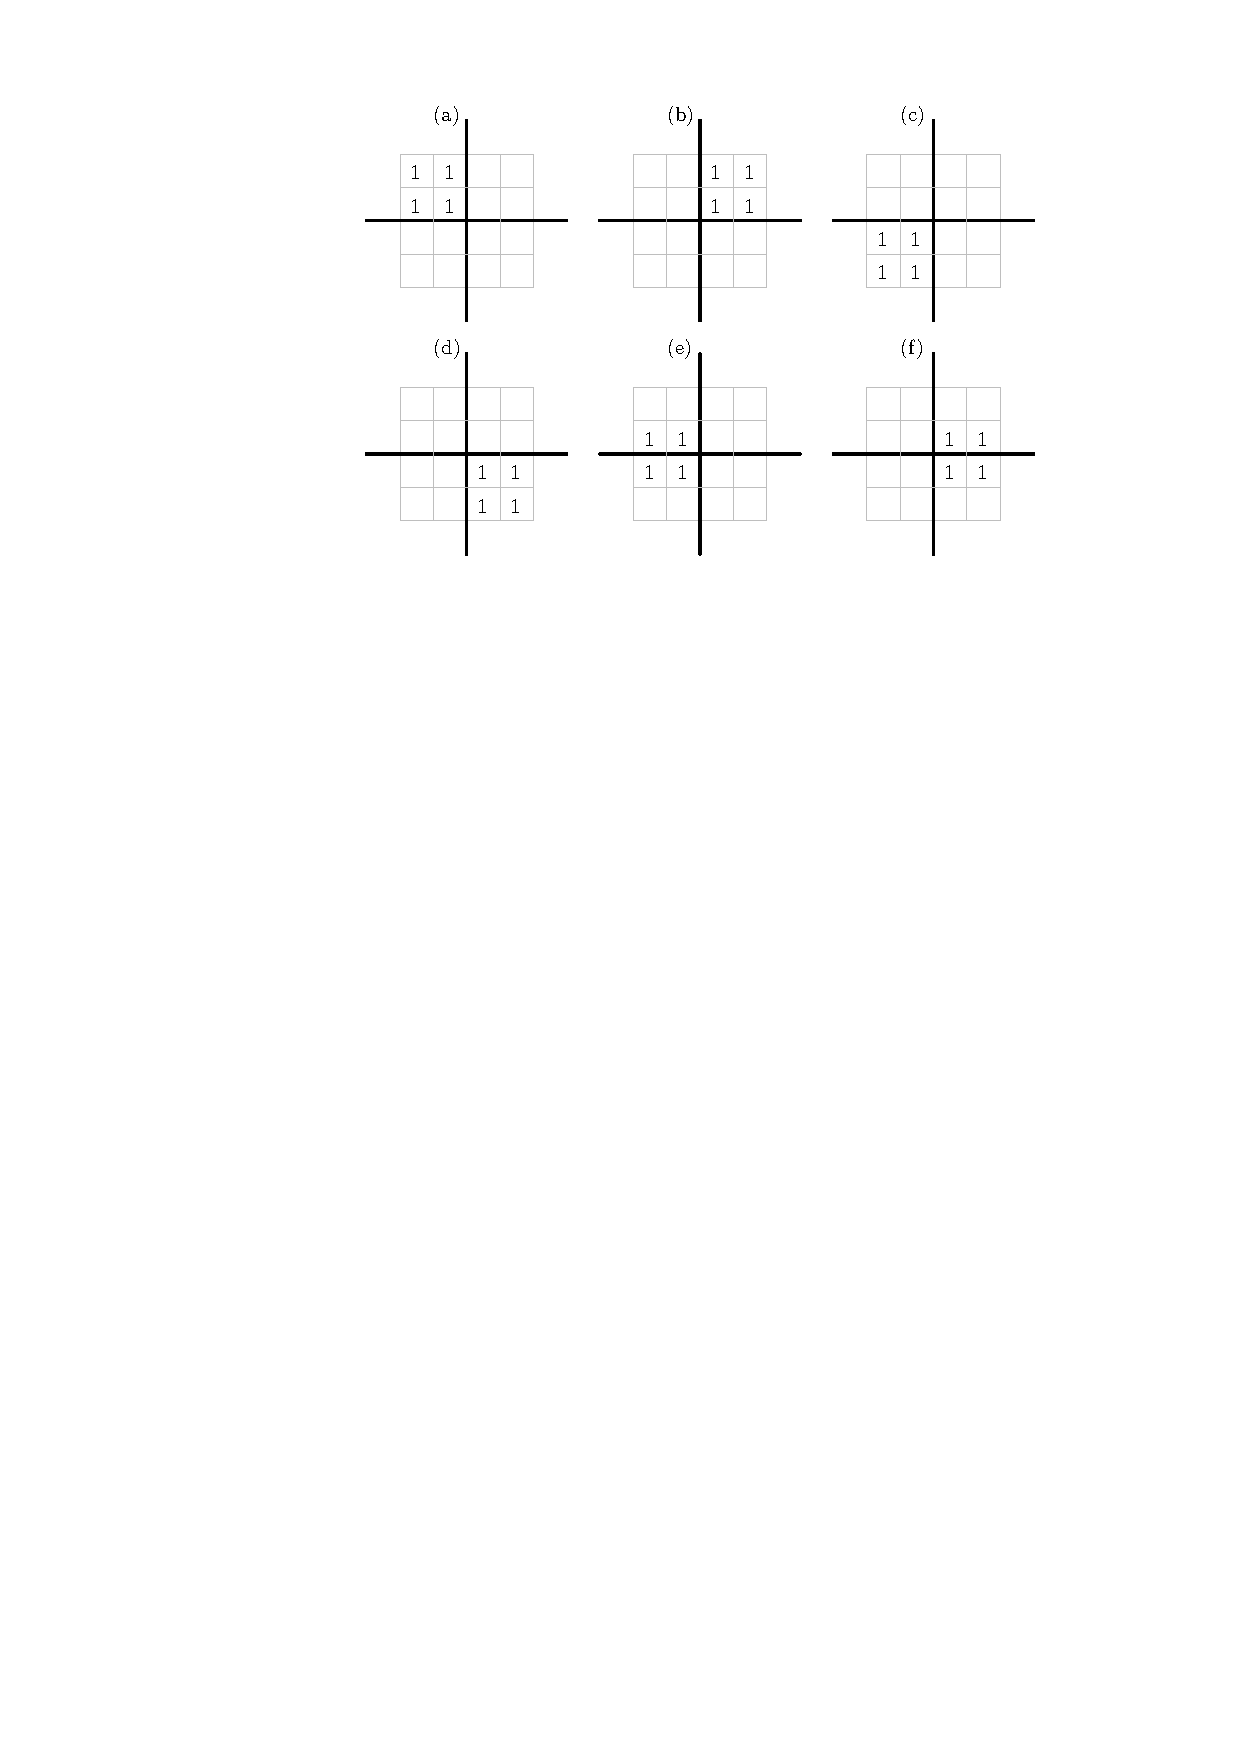
\includegraphics[width=0.9\textwidth]{fig/Q_bunos_1.pdf}
	\label{img7_b}
\end{figure}


حالا هرکدام از این حالت‌ها را به عنوان یک تابع درنظر می‌گیریم و برای قسمت (آ) جدول درستی آن را می‌نویسیم:



\begin{latin}
	\centering
	\[
	\begin{array}{|c|c|c|c|c|c|c|c|c|c|}
		\hline
		A & B & C & D & f_a & f_b & f_c & f_d & f_e & f_f \\
		\hline\hline
		0 & 0 & 0 & 0 & 1 & 0 & 0 & 0 & 0 & 0 \\
		0 & 0 & 0 & 1 & 1 & 0 & 0 & 0 & 1 & 0 \\
		0 & 0 & 1 & 0 & 0 & 0 & 1 & 0 & 0 & 0 \\
		0 & 0 & 1 & 1 & 0 & 0 & 1 & 0 & 1 & 0 \\
		0 & 1 & 0 & 0 & 1 & 0 & 0 & 0 & 0 & 0 \\
		0 & 1 & 0 & 1 & 1 & 0 & 0 & 0 & 1 & 0 \\
		0 & 1 & 1 & 0 & 0 & 0 & 1 & 0 & 0 & 0 \\
		0 & 1 & 1 & 1 & 0 & 0 & 1 & 0 & 1 & 0 \\
		1 & 0 & 0 & 0 & 0 & 1 & 0 & 0 & 0 & 0 \\ 
		1 & 0 & 0 & 1 & 0 & 1 & 0 & 0 & 0 & 1 \\
		1 & 0 & 1 & 0 & 0 & 0 & 0 & 1 & 0 & 0 \\
		1 & 0 & 1 & 1 & 0 & 0 & 0 & 1 & 0 & 1 \\
		1 & 1 & 0 & 0 & 0 & 1 & 0 & 0 & 0 & 0 \\
		1 & 1 & 0 & 1 & 0 & 1 & 0 & 0 & 0 & 1 \\
		1 & 1 & 1 & 0 & 0 & 0 & 0 & 1 & 0 & 0 \\
		1 & 1 & 1 & 1 & 0 & 0 & 0 & 1 & 0 & 1 \\
		\hline
	\end{array}
	\]
\end{latin}


خروجی ساده نشده توابع به‌صورت زیر می‌شود:

\begin{latin}
	\begin{enumerate}
		\item 
		$f_a=A'B'C'D' + A'B'C'D + A'BC'D' + A'BC'D$
		
		\item 
		$f_b=AB'C'D' + AB'C'D + ABC'D' + ABC'D$
		
		\item 
		$f_c=A'B'CD' + A'B'CD + A'BCD' + A'BCD$
		
		\item 
		 $f_d=AB'CD' + AB'CD + ABCD' + ABCD$
		 
		 \item 
		 $f_e=A'B'C'D + A'B'CD + A'BC'D + A'BCD$
		 
		 \item 
		 $f_f=AB'C'D + AB'CD + ABC'D + ABCD$
	\end{enumerate}
\end{latin}


حالا هرکدام از این حالت‌ها را به‌عنوان یک جدول کارنو ۴ ورودی با ورودی‌های A و B و C و D درنظر می‌گیریم. و تابع ساده شده برای هریک را به‌دست می‌آوریم:


\begin{latin}
	\begin{enumerate}
		\item 
		$f_a=A'C'$
		
		\item 
		$f_b=AC'$
		
		\item 
		$f_c=A'C$
		
		\item 
		$f_d=AC$
		
		\item 
		$f_e=A'D$
		
		\item 
		$f_f=AD$
	\end{enumerate}
\end{latin}

و درنهایت یکی از مدار‌های ممکن برای این سوال را می‌توان به‌صورت زیر رسم نمود:

\begin{figure}[h]
	\centering
	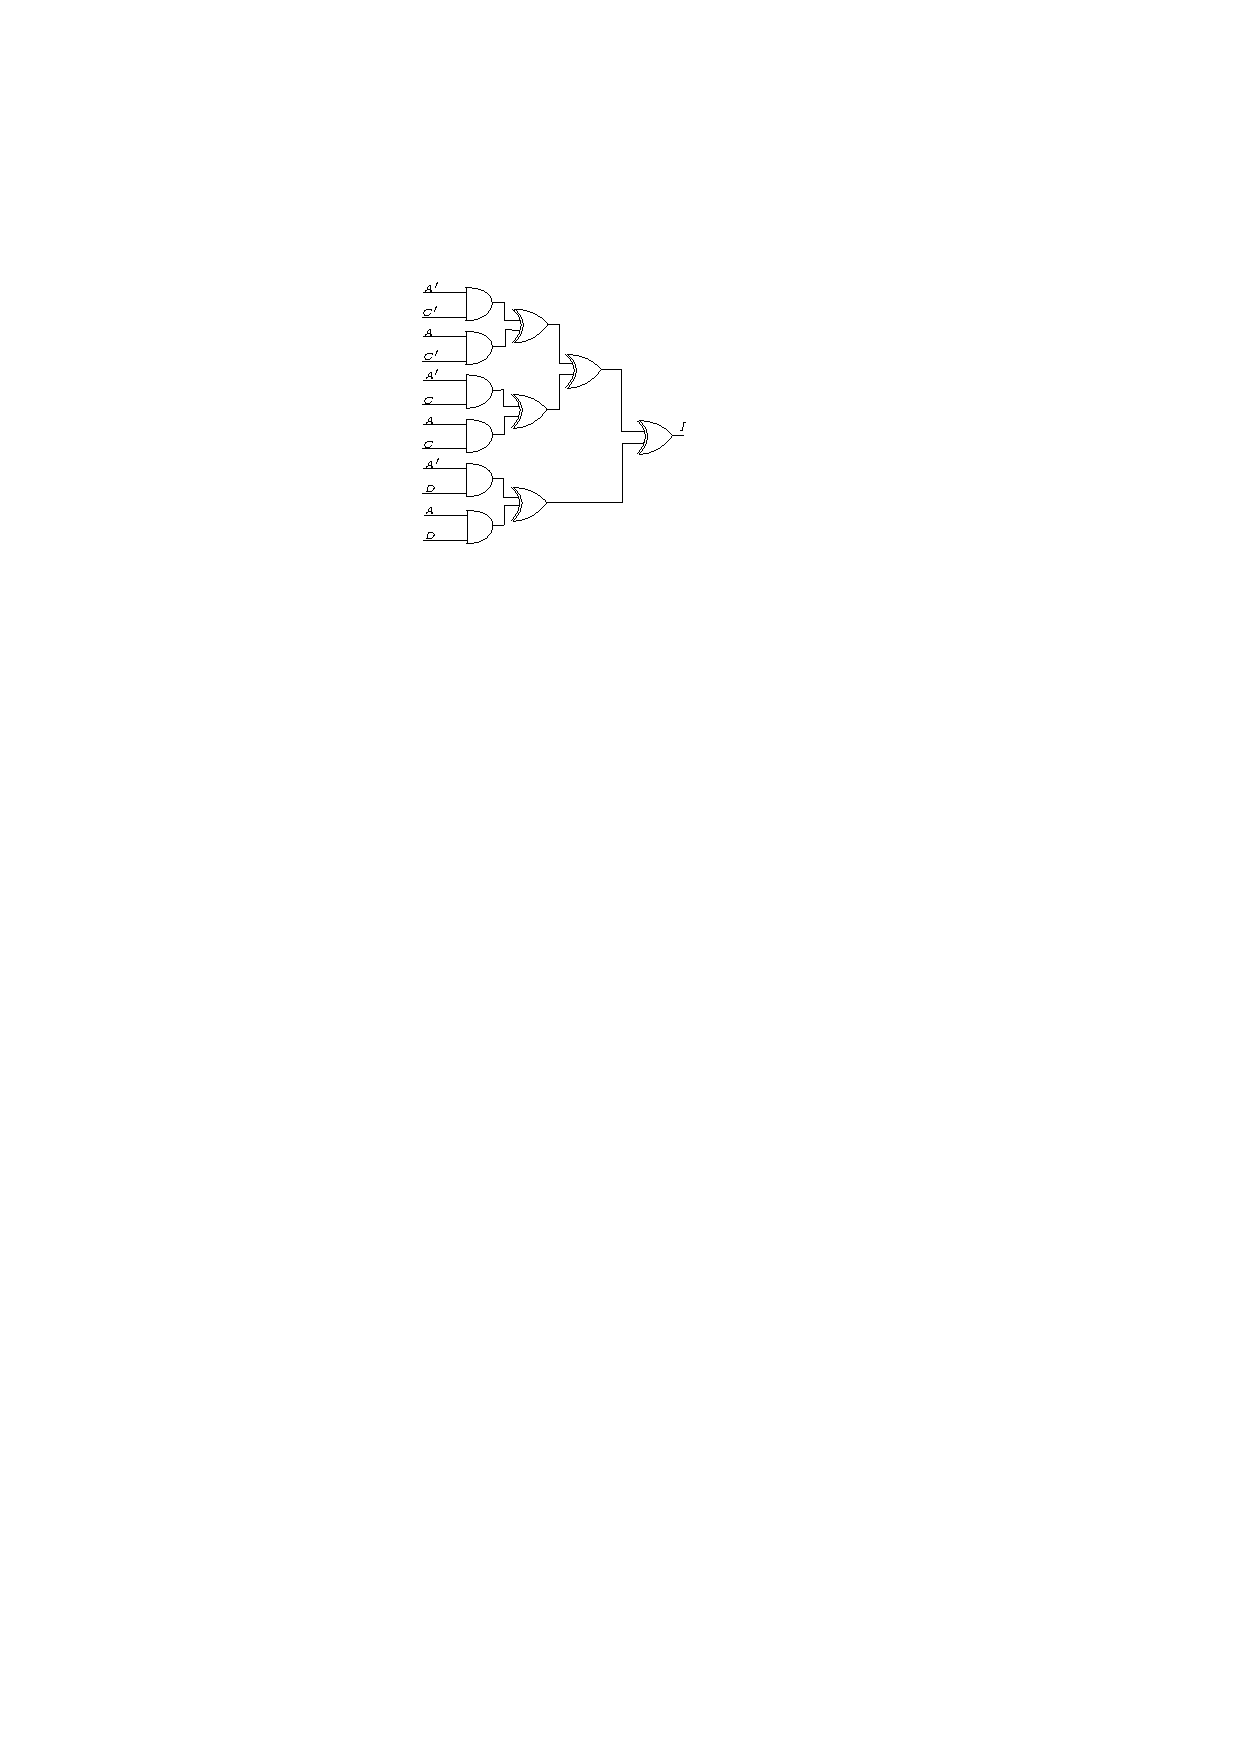
\includegraphics[width=0.5\textwidth]{fig/Q_bunos_circ.pdf}
	\label{img1_bunus}
\end{figure}


این مدار صرفا یک مربع را در تصویر تشخیص می‌دهد، اما نمی‌تواند محل مربع را تعیین کند. درصورت اینکه نیاز به تعیین محل مربع داشتیم، می‌بایست در خروجی گیت‌های \lr{AND} از یک \lr{Decoder} استفاده کنیم.

توضیحات داده شده برای زمانی بود که مربع‌ها را با ۱ تشخیث بدهیم. در صورت سوال گفته شده است مربع‌ها را با مقدار پیکسل ۰ هم باید قابل تشخیص باشند. برای حل این قسمت تنها کافیست مراحل گفته شده را با مقدار صفر برای هر پیکسل (از بین ۶ حالت مجاز) تکرار کنید.

